\documentclass[10pt,twocolumn,letterpaper]{article}

\usepackage{cvpr}
\usepackage{times}
\usepackage{epsfig}
\usepackage{graphicx}
\usepackage{amsmath}
\usepackage{amssymb}
\usepackage[utf8x]{inputenc}
\renewcommand{\refname}{Bibliografia}
\usepackage{listings}
\renewcommand{\lstlistingname}{}
\renewcommand{\figurename}{Figura}


\usepackage{url}

% Include other packages here, before hyperref.

% If you comment hyperref and then uncomment it, you should delete
% egpaper.aux before re-running latex.  (Or just hit 'q' on the first latex
% run, let it finish, and you should be clear).
%\usepackage[pagebackref=true,breaklinks=true,letterpaper=true,colorlinks,bookmarks=false]{hyperref}

\cvprfinalcopy % *** Uncomment this line for the final submission

\def\cvprPaperID{****} % *** Enter the CVPR Paper ID here
\def\httilde{\MBox{\tt\raisebox{-.5ex}{\syMBol{126}}}}

% Pages are nuMBered in submission mode, and unnuMBered in camera-ready
\ifcvprfinal\pagestyle{empty}\fi
\begin{document}

%%%%%%%%% TITLE
\title{Parallel Computing Final\\BigramTrigramGenerator con Java, Java Threads \& C++ Threads}

\maketitle
\thispagestyle{empty}

%%%%%%%%% ABSTRACT
\begin{abstract}
L'obiettivo di questo progetto è quello di calcolare tutte le occorrenze di bigrammi e trigrammi di lettere presenti all'interno di un testo. In questa relazione verranno presentati e successivamente confrontati tre approcci diversi: uno sequenziale (in Java) e due paralleli (con Java Thread e C++ Thread).
\end{abstract}

%%%%%%%%% BODY TEXT
\section{Introduzione}
Un algoritmo che ricerca bigrammi e trigrammi di lettere o, più in generale, un algoritmo che esegue delle computazioni indipendenti su ciascuna riga di un file testo fa parte della classe di problemi che si prestano meglio alla parallelizzazione: due o più thread possono lavorare nello stesso momento su porzioni del testo differenti, per poi unire tutti i risultati alla fine.
   
\subsection{Bigrammi \& Trigrammi}
In generale un \textit{n-gramma} è una sottosequenza di n elementi di una data sequenza; gli elementi in questione possono essere sillabe, lettere, parole, ecc \cite{N-GRAMMA}. Per questo progetto ci siamo occupati di n-grammi di lettere. In particolare:
\begin{itemize}
	\item Una sequenza di due lettere si dice \textit{bigramma} (o \textit{digramma})
	\item Una sequenza di tre lettere si dice \textit{trigramma}
\end{itemize}

\subsection{Descrizione del dataset}
Il dataset utilizzato è stato estratto dal database del \textit{Progetto Gutenberg}, una biblioteca digitale di eBook di pubblico dominio, liberamente riproducibili e scaricabili \cite{GUTENBERG}. 

Il testo scelto è \textit{"La scienza in cucina e l'arte di mangiar bene"} di Pellegrino Artusi \cite{ARTUSI}. Per eseguire i vari esperimenti, il testo è stato accorciato ed allungato in modo da ottenere file di dimensioni diverse: 50kb, 100kb, 200kb, 500kb, 1MB, 2MB, 4MB, 8MB, 16MB, 32MB.

\subsection{Specifiche Hardware}
Per questi esperimenti è stato utilizzato un MacBook Pro (Retina, 13-inch, Mid 2014) con le seguenti specifiche:
\begin{itemize}
	\item Processore 2,6 GHz Dual-Core Intel Core i5
	\item Memoria 8 GB 1600 MHz DDR3
	\item Memoria Flash Storage 128 GB
\end{itemize}

\section{Implementazione}
Sono state eseguite tre implementazioni, una in maniera sequenziale in linguaggio Java e due in maniera parallela rispettivamente con Java Thread e C++ Thread.

\subsection{Versione Sequenziale in Java}
La versione sequenziale dell'algoritmo è piuttosto semplice. Per prima cosa è stata creata una classe, \textit{LinesExtractor}, che prende in input il nome del file \textit{txt} ed espone un metodo, \textit{extractLines}, che legge il file e restituisce una lista di tutte le righe del testo, escludendo per semplicità righe vuote e caratteri speciali. L'estrazione delle righe avviene tramite il metodo \textit{readAllLines} della classe \textit{Files} della libreria standard di Java. La rimozione di caratteri speciali è stata eseguita con un'espressione regolare.\newline

\begin{lstlisting}[basicstyle=\scriptsize, language=Java, frame=single, caption={Esempio di estrazione di righe da un file in Java},captionpos=b, showstringspaces=false, mathescape=true]
public List<String> extractLines() {
  
  List<String> finalLines = new ArrayList<>();
  List<String> lines = null;
  String regex = "[$\hat{}$A-Za-z0-9' ]";

  FileSystem fs = FileSystems.getDefault();
  lines = Files.readAllLines(fs.getPath("", filename));
  lines.forEach(line -> {
    if (!line.isBlank() && !line.isEmpty()) {
      line = line.toLowerCase().replaceAll(regex, "");
      finalLines.add(line);
    }
  });
  
  return finalLines;
}  
\end{lstlisting}

La funzione principale prende in input la lista di righe ed estrae una nuova lista contenente tutte le parole al suo interno. L'estrazione di parole è stata implementata con un'altra espressione regolare (\textit{\textbackslash \textbackslash s+}). \newline

\begin{lstlisting}[basicstyle=\scriptsize, language=Java, frame=single, caption={Esempio di estrazione di parole in Java},captionpos=b, showstringspaces=false]
LinesExtractor extractor = new LinesExtractor(filename);
List<String> lines = extractor.extractLines();

List<String> words = new ArrayList<>();
lines.forEach(line -> {
  words.addAll(Arrays.asList(line.split("\\s+")));
});

words.removeAll(Collections.singleton(""));
\end{lstlisting}

A questo punto vengono calcolati i bigrammi o i trigrammi su ognuna delle parole estratte, utilizzando il metodo \textit{substring} della classe \textit{String} della libreria standard di Java. Il tempo di esecuzione viene misurato con la funzione \textit{currentTimeMillis()} della libreria standard \textit{System}.\newline

\begin{lstlisting}[basicstyle=\scriptsize, language=Java, frame=single, caption={Esempio di ricerca di bigrammi/trigrammi in Java},captionpos=b, showstringspaces=false]
long start = System.currentTimeMillis();

int n = 2; // 2: bigrammi, 3: trigrammi

List<String> ngrams = new ArrayList<>();
for (String word: words) {
  if (word.length() >= n) {
    for (int i = 0; i < word.length() - (n - 1); i++) {
      ngrams.add(word.substring(i, i + n));
    }
  }
}

long end = System.currentTimeMillis();
\end{lstlisting}

\subsection{Versione Parallela con Java Thread}
Per la versione parallela con Java Thread è stata utilizzata la stessa classe \textit{LinesExtractor} (come per la versione sequenziale) per estrarre le righe dal testo, ed è uguale anche la procedura con cui vengono estratte le parole.

Per il conteggio dei bigrammi o trigrammi è stata utilizzata una variabile  \textit{globalCounter} di tipo \textit{AtomicInteger}, condivisa tra tutti i thread, in modo che ogni thread possa aggiornarla evitando inconsistenze.

È stata quindi creata una classe, \textit{NGramThread}, che estende la classe \textit{Thread} e il suo costruttore riceve in ingresso:
\begin{itemize}
	\item \textit{globalCounter}: riferimento alla variabile di tipo \textit{AtomicInteger}, rappresenta il contatore globale del numero di \textit{n-grammi} trovati
	\item \textit{words}: l'intera lista di parole
	\item \textit{n}: intero che specifica se vengono trattati bigrammi (\textit{n=2}) oppure trigrammi (\textit{n}=3)
	\item \textit{start} e \textit{stop}: due interi che indicano gli indici di partenza e arrivo del range di parole su cui ciascun thread lavora
\end{itemize}

Appena il thread viene lanciato, viene eseguita la funzione \textit{run()} che si occupa del calcolo degli \textit{n-grammi}.

La classe presenta anche un intero privato, \textit{nGramCounter}, inizializzato a zero e che viene incrementato ad ogni \textit{n-gramma} trovato. Una volta calcolati tutti gli \textit{n-grammi} sul range di parole, si aggiorna il valore dell'intero atomico \textit{globalCounter} tramite la funzione \textit{addAndGet} della classe \textit{AtomicInteger} nel package \textit{java.util.concurrent.Atomic}, aggiungendo in maniera atomica il valore di \textit{nGramCounter}. Questo viene fatto per ridurre al minimo il numero di operazioni atomiche da eseguire in ogni thread.\newline

\begin{lstlisting}[basicstyle=\scriptsize, language=Java, frame=single, caption={Esempio di ricerca di bigrammi/trigrammi con Java Thread},captionpos=b]
public class NGramThread extends Thread {

  private int n, start, stop;
  private List<String> words;
  private AtomicInteger globalCounter;
  private int nGramCounter = 0;

  public void run() {
    if (stop > words.size()) stop = words.size();
    List<String> ngrams = new ArrayList<>();
    for (int i=start; i<stop; i++) {
      String word = words.get(i);
      for (int j = 0; j < word.length() - (n-1); j++) {
        ngrams.add(word.substring(j, j+n));
        nGramCounter++;
      }
    }
    globalCounter.addAndGet(nGramCounter);
  }
}
\end{lstlisting}
Nel main vengono quindi lanciati un numero variabile di thread, e ne viene fatto il \textit{join} per aspettare che terminino l'esecuzione. 
Anche in questo caso il tempo di esecuzione viene misurato con la funzione \textit{currentTimeMillis()} della libreria standard \textit{System}.\newline

\begin{lstlisting}[basicstyle=\scriptsize, language=Java, frame=single, caption={Lancio di Java Thread per ricerca di bigrammi/trigrammi},captionpos=b]
AtomicInteger gCounter = new AtomicInteger(0);
List<NGramThread> threads = new ArrayList<>();
int blockSize = words.size()/numThreads+1;
int n = 2; // 2: bigrammi, 3: trigrammi
int i = 0;

long start = System.currentTimeMillis();

while (i < numThreads) {
  int s = i*blockSize; // indice partenza
  int e = (i+1)*blockSize; // indice arrivo
  threads.add(new NGramThread(gCounter,words,n,s,e));
  threads.get(i).start();
  i++;
}

for (NGramThread worker: threads) {
  worker.join();
}

long end = System.currentTimeMillis();
\end{lstlisting}

\subsection{Versione Parallela con C++ Thread}
Per la versione parallela con C++ Thread è stata creata una classe \textit{LinesExtractor}, equivalente della versione in Java, che prende in input il nome del file \textit{txt} ed espone un metodo, \textit{extractLines}, che legge il file e restituisce un vettore di stringhe, una per ogni riga estratta dal testo (escludendo per semplicità righe vuote e caratteri speciali). L'estrazione delle righe avviene tramite la funzione \textit{getline} della classe \textit{ifstream} della libreria standard del C++.

Anche in questo caso la rimozione di caratteri speciali è stata eseguita con un’espressione regolare.\newline

\begin{lstlisting}[basicstyle=\scriptsize, language=C++, frame=single, caption={Esempio di estrazione di righe da un file in C++},captionpos=b,showstringspaces=false, mathescape=true]
vector<string> extractLines() {

    vector<string> lines;
    string line;
    
    ifstream file(filename);

    if (!file) {
        throw runtime_error("Could not open file!");
    }

    regex reg("[$\hat{}$A-Za-z0-9' ]");

    while (getline(file, line)) {
        transform(line.begin(), line.end(), ::tolower);
        string cleaned = regex_replace(line, reg, "");
        if (!cleaned.empty()) {
            lines.push_back(cleaned);
        }
    }

    file.close();
    return lines;
}
\end{lstlisting}

La funzione principale prende in input la lista di righe ed estrae una nuova lista contenente tutte le parole al suo interno. L'estrazione di parole è stata implementata utilizzando la classe \textit{stringstream} e l'iteratore \textit{istream\_iterator}.\newline

\begin{lstlisting}[basicstyle=\scriptsize, language=Java, frame=single, caption={Esempio di estrazione di parole in C++},captionpos=b, showstringspaces=false]
LinesExtractor extractor(filename);
vector<string> lines = extractor.extractLines();
vector<string> words;

for (auto &line: lines) {
  stringstream ss(line);
  istream_iterator<string> begin(ss), end;
  vector<string> lineWords(begin, end);
  
  for (auto &word: lineWords) {
    if (!word.empty()) { 
      words.push_back(word);
    }
  }
  
}
\end{lstlisting}

Per il conteggio dei bigrammi o trigrammi è stato utilizzata una variabile \textit{globalCounter} di tipo \textit{atomic\_int}, condivisa tra tutti i thread, in modo che ogni thread possa aggiornarla evitando inconsistenze.

La classe \textit{thread} della libreria standard del C++ (\textit{std::thread}), introdotta con C++11, richiede nel costruttore un oggetto \textit{callable} (riferimento a funzione o laMBda expression), porzione di codice che viene eseguita non appena il thread viene lanciato.
È stata quindi creata una funzione \textit{run()} per il calcolo degli \textit{n-grammi} che riceve in ingresso:
\begin{itemize}
	\item \textit{globalCounter}: riferimento alla variabile di tipo \textit{atomic\_int}, rappresenta il contatore globale del numero di \textit{n-grammi} trovati
	\item \textit{words}: l'intero vettore di parole
	\item \textit{n}: intero che specifica se vengono trattati bigrammi (\textit{n}=2) oppure trigrammi (\textit{n}=3)
	\item \textit{start} e \textit{stop}: due interi che indicano gli indici di partenza e di arrivo del range di parole su cui ciascun thread lavora
\end{itemize}

La funzione \textit{run()} al suo interno instanzia un intero, \textit{nGramCounter}, inizializzato a zero e che viene incrementato ad ogni \textit{n-gramma} trovato. Una volta calcolati tutti gli \textit{n-grammi} sul range di parole, si aggiorna il valore dell'intero atomico \textit{globalCounter} tramite la funzione \textit{fetch\_add} della libreria \textit{std::atomic}, aggiungendo in maniera atomica il valore di \textit{nGramCounter}. Come per la versione parallela con Java Thread, questo viene fatto per ridurre al minimo il numero di operazioni atomiche da eseguire in ogni thread.\newline

\begin{lstlisting}[basicstyle=\scriptsize, language=C++, frame=single, caption={Esempio di funzione lanciata da un thread in C++},captionpos=b,showstringspaces=false]
void run(atomic_int& counter, int id, int n,
         vector<string> words, int start, int stop) {

  int nGramCounter = 0;

  if (stop > words.size()) stop = words.size();

  vector<string> ngrams;
  for (int i=start; i<stop; i++) {
    string word = words[i];
    if (word.length() >= n) {
      for (int j=0; j<word.length()-(n-1); j++) {
        ngrams.push_back(word.substr(j, n));
        nGramCounter++;
      }
    }
  }

  counter.fetch_add(nGramCounter, memory_order_relaxed);
}
\end{lstlisting}

Nel main vengono quindi lanciati un numero variabile di thread, e ne viene fatto il join per aspettare che terminino l’esecuzione.

Il tempo di esecuzione è stato misurato utilizzando il metodo \textit{now()} della classe \textit{steady\_clock} della libreria \textit{chrono}. La classe \textit{steady\_clock} rappresenta un \textit{clock} di tipo \textit{monotonic} e il suo funzionamento è simile a quello di un \textit{wall-clock}, ideale per misurare intervalli di tempo in un thread (a differenza del tempo di CPU, che misurerebbe il tempo totale speso in tutti i thread).
\newpage

\begin{lstlisting}[basicstyle=\scriptsize, language=C++, frame=single, caption={Lancio di C++ Thread per la ricerca di bigrammi/trigrammi},captionpos=b,showstringspaces=false]
int blockSize = words.size() / numThreads + 1;
atomic_int globalCounter(0);

int n = 2; // 2: bigrammi, 3: trigrammi

auto start = chrono::steady_clock::now();

std::vector<thread> threads(numThreads);
for (int i = 0; i < numThreads; i++) {
  int s = i*blockSize; // indice partenza
  int e = (i+1)*blockSize; // indice arrivo
  threads[i] = thread(run, ref(globalCounter), 
                      i, n, words, s, e);
}
for (auto &th: threads) {
  th.join();
}

auto end = chrono::steady_clock::now();
chrono::duration<double> elapsedSeconds = end - start;
\end{lstlisting}

\section{Esperimenti \& Risultati}
Per ogni esperimento sono state eseguite cinque iterazioni in modo da ottenere un misura più accurata dei risultati.
Tutti i grafici presentati di seguito sono stati generati con uno script Python utilizzando la libreria \textit{matplotlib}.

L’accuratezza dei risultati ottenuti è stata valutata tramite metrica dello \textit{Speedup} (S), definito come il rapporto tra il tempo di esecuzione sequenziale ($t_s$) e il tempo di esecuzione parallelo ($t_p$): $S = \frac{t_s}{t_p}$.

\subsection{Valutazione dello speedup con Java Thread}
Viste le risorse hardware, è stato scelto di eseguire gli esperimenti con 2 o 4 thread.
Una volta scelto il testo \textit{"La scienza in cucina e l'arte di mangiar bene"} di Pellegrino Artusi, è stato quindi misurato lo \textit{speedup} al variare delle dimensioni del file di testo (50kb, 100kb, 200kb, 500 kb, 1MB, 2MB, 4MB, 8MB, 16MB, 32MB).

Come si può notare dalle immagini lo speedup risulta essere maggiore di 1 oltre una certa soglia ($\approx$ 100kb per i bigrammi e  $\approx$ 500kb per i trigrammi).

\begin{figure}[h]
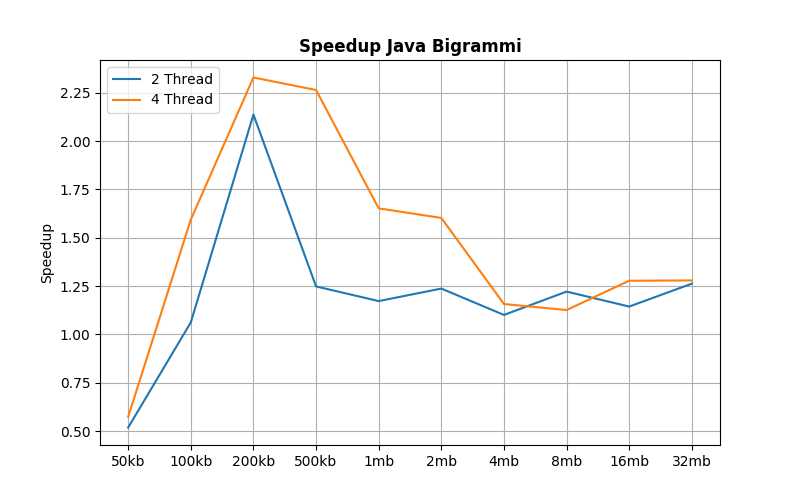
\includegraphics[width=\linewidth]{Plots/speedup_java_bigrammi.png}
\caption{Speedup bigrammi con Java Thread}
\end{figure}

\begin{figure}[h]
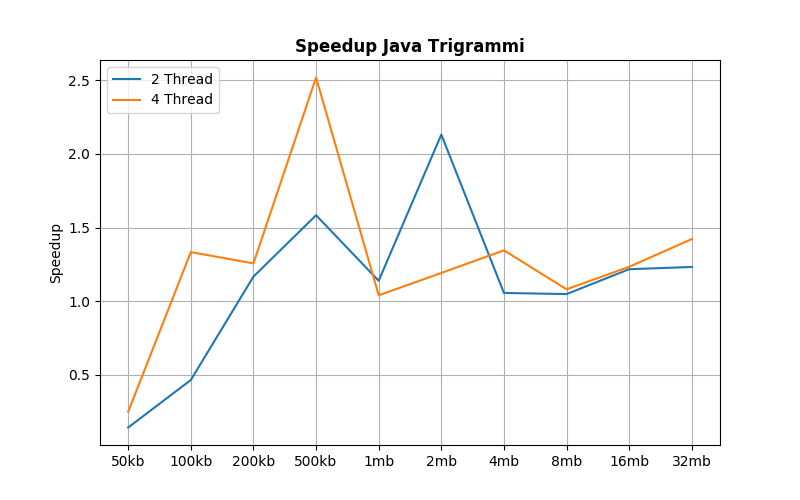
\includegraphics[width=\linewidth]{Plots/speedup_java_trigrammi.png}
\caption{Speedup trigrammi con Java Thread}
\end{figure}

\newpage
\subsection{Valutazione dello speedup con C++ Thread}
Anche in questo caso è stato scelto di utilizzare 2 o 4 thread.
Come si può notare dalle immagini, dopo una certa soglia ($\approx$ 16 MB) c'è un aumento significativo dello \textit{speedup}. È ragionevole pensare che aumentando ulteriormente la dimensione del file, si possa ottenere uno \textit{speedup} ancora maggiore.

\begin{figure}[h]
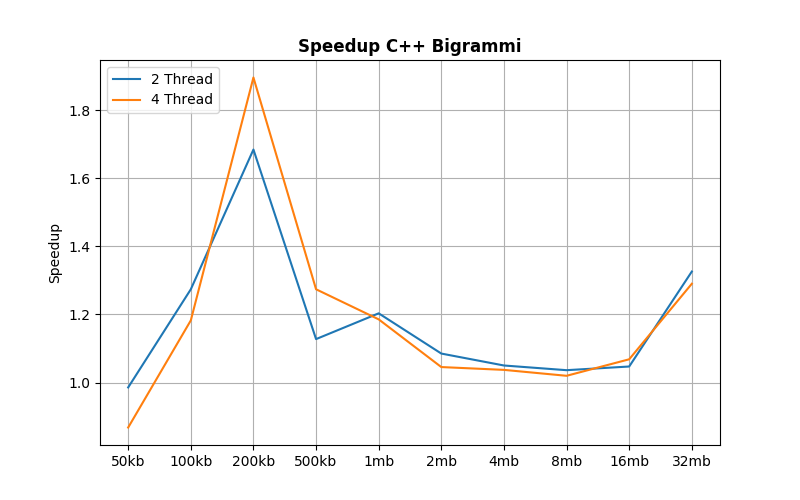
\includegraphics[width=\linewidth]{Plots/speedup_cpp_bigrammi.png}
\caption{Speedup Bigrammi con C++ Thread}
\end{figure}

\begin{figure}[h]
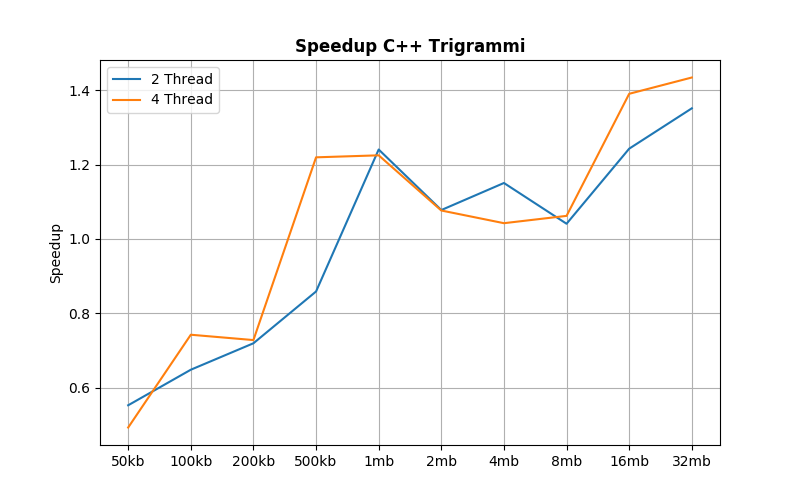
\includegraphics[width=\linewidth]{Plots/speedup_cpp_trigrammi.png}
\caption{Speedup Trigrammi con C++ Thread}
\end{figure}
\newpage

\newpage
\subsection{Confronto sui tempi di esecuzione con Java Thread}
Per avere dei risultati più accurati, è stato eseguito un confronto anche sui tempi di esecuzione con Java Thread rispetto alla versione sequenziale.

Come si può chiaramente notare dai risultati ottenuti, da una certa dimensione in poi ($\approx$ 4MB) gli approcci paralleli risultano sempre più efficienti rispetto all'approccio sequenziale. Non sono state riscontrare differenze sostanziali tra l'utilizzo di 2 o 4 thread.
\begin{figure}[h]
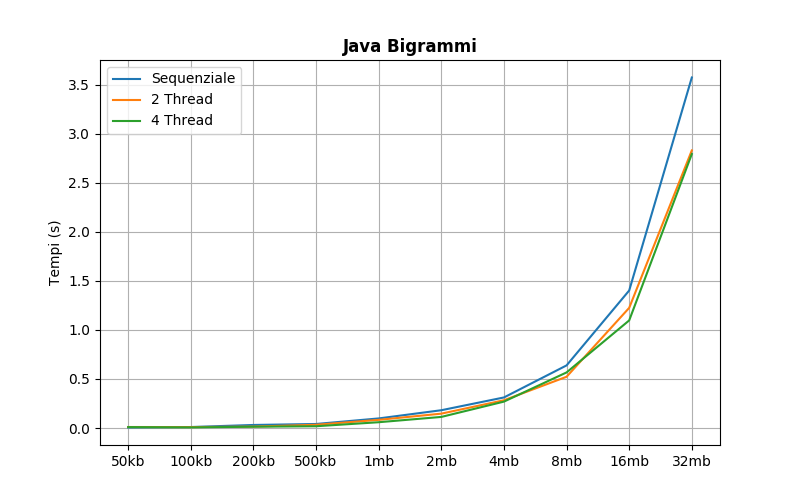
\includegraphics[width=\linewidth]{Plots/tempi_java_bigrammi.png}
\caption{Confronto tempi di esecuzione bigrammi Java}
\end{figure}

\begin{figure}[h]
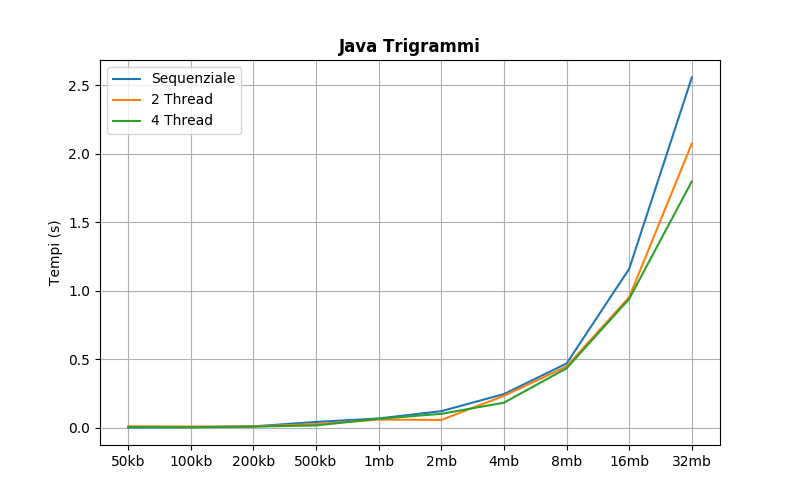
\includegraphics[width=\linewidth]{Plots/tempi_java_trigrammi.png}
\caption{Confronto tempi di esecuzione trigrammi Java}
\end{figure}

\subsection{Confronto sui tempi di esecuzione con C++ Thread}
Allo stesso modo è stato eseguito un confronto anche sui tempi di esecuzione con C++ Thread rispetto alla versione sequenziale.
Come si può notare dai risultati ottenuti, molto simili ai precedenti, anche in questo caso da una certa dimensione in poi ($\approx$ 8 MB) gli approcci paralleli risultano sempre più efficienti rispetto all'approccio sequenziale.
\begin{figure}[h]
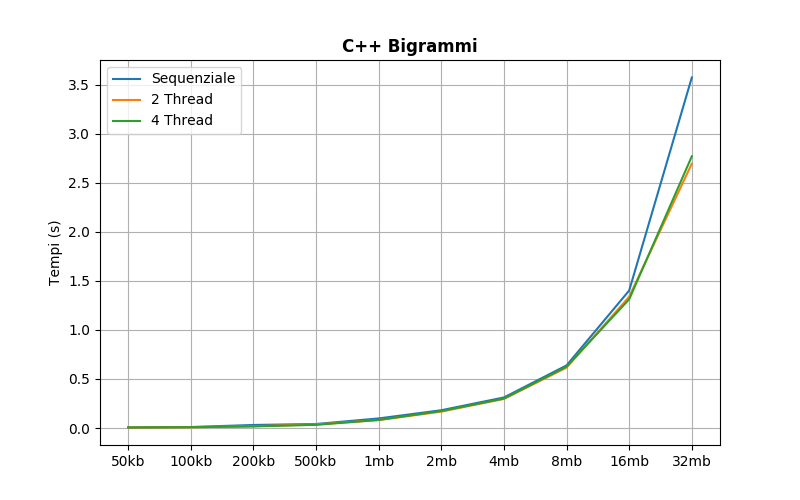
\includegraphics[width=\linewidth]{Plots/tempi_cpp_bigrammi.png}
\caption{Confronto tempi di esecuzione Bigrammi C++}
\end{figure}

\begin{figure}[h]
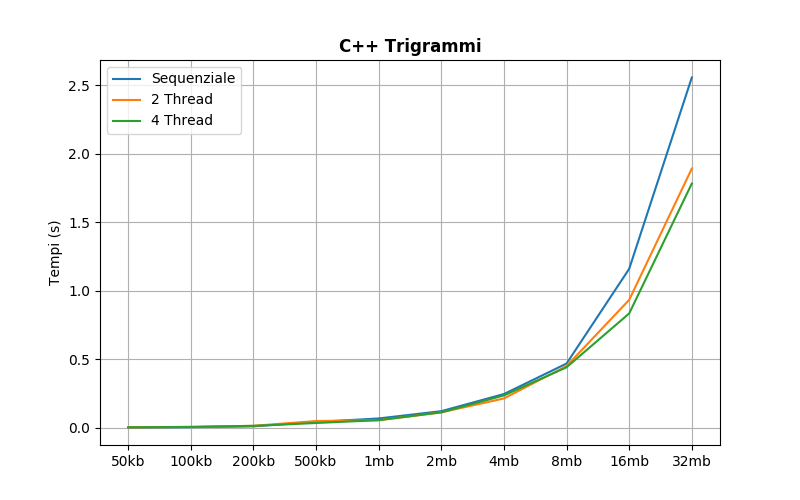
\includegraphics[width=\linewidth]{Plots/tempi_cpp_trigrammi.png}
\caption{Confronto tempi di esecuzione Trigrammi C++}
\end{figure}

\section{Conclusione}
Come era possibile aspettarsi per file di grosse dimensioni l'approccio parallelo è sempre migliore di quello sequenziale: più lungo è il testo è maggiore sarà lo \textit{speedup} ottenuto.

In generale l'implementazione in Java è risultata più veloce, considerando anche il fatto che non negli esperimenti non è stato incluso il tempo di estrazione di righe e parole, che risulta essere significativamente maggiore (circa 3 volte) con C++ rispetto al Java.

{
\bibliographystyle{unsrt}
\bibliography{bibliografia.bib}
}


\end{document}
